\documentclass[oneside]{mgr}
% \documentclass[12pt]{article}
% \usepackage[margin=25mm]{geometry}
\usepackage[T1]{fontenc}
\usepackage{mathptmx}
\usepackage[utf8]{inputenc}
\usepackage{graphicx}
\graphicspath{ {img/} }
\usepackage{url}
\usepackage[figurename=Ilustracja]{caption}

\author{Mateusz Korzeniowski}
\title{Aplikacja webowa wspomagająca planowanie wyjazdu turystycznego, według wzorca architektonicznego Serverless}
\engtitle{Web based application supporting planning of tourist travel, built using Serverless architectural pattern}
\supervisor{dr inż. Paweł Stelmach, Katedra Informatyki na Wydziale Informatyki i Zarządzania}
\field{Informatyka}
\specialisation{-}
\date{2017}

\renewcommand{\contentsname}{Spis treści}
\renewcommand{\chaptername}{Rozdział}
\renewcommand{\bibname}{Bibliografia}

\begin{document}
\maketitle
% \dedication{6cm}{Rodzicom}
\tableofcontents

\chapter{Wstęp}
Rozwój oprogramowania komputerowego od swych początków opierał się na procesie budowania kolejnych, nakładających się na siebie warstw oprogramowania, które pozwalały coraz bardziej abstrahować od problemów niskiego poziomu, związanych ze sposobem działania samych komputerów. Pozwoliło to programistom skupić się na projektowaniu coraz bardziej złożonych i finezyjnych programów bez potrzeby skupiania się na komunikacji pomiędzy komponentami fizycznego systemu komputerowego, na którym ich program jest uruchomiony.

Doskonałą analogią budowy zaawansowanego oprogramowania systemów komputerowych jest stos komunikacyjny protokołu TCP/IP, gdzie kolejne warstwy posiadają ściśle określone role, a programy wykorzystujące warstwy wyższe - bardziej oddalone od fizycznego medium - nie muszą brać pod uwagę problemów i zjawisk, z którymi borykają się warstwy pod nimi.

\begin{figure}
	\centering
	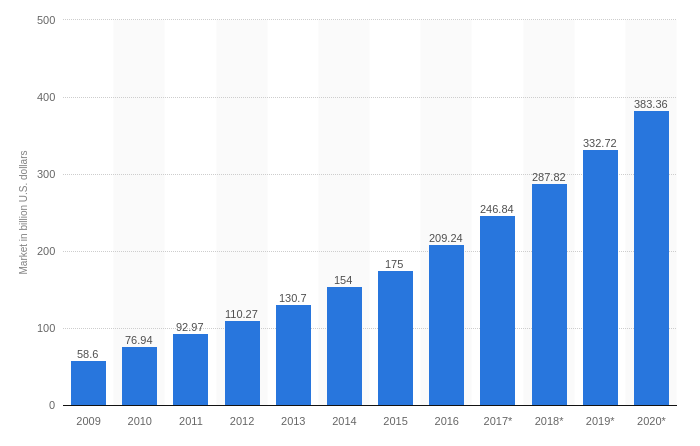
\includegraphics[width=15cm]{2017-03-1910:36:22}
	\caption{Rozmiar rynku usług chmurowych oraz prognoza do roku 2020 w miliardach dolarów amerykańskich \cite{statisticCloudComputingMarketSize}}
	\label{fig:cloudComputingMarketSize}
\end{figure}

Współcześnie podobny trend obserwować możemy w kwestii oddalania się przedsiębiorstw zajmujących się wytwarzaniem oprogramowania od warstwy sprzętowej środowiska, w którym ich aplikacje będą działać. O ile jeszcze dekadę temu firmy informatyczne zazwyczaj posiadały własne, fizyczne serwery służące do testowania i uruchamiania aplikacji, wraz z personelem potrzebnym do utrzymania i zarządzania taką infrastrukturą, o tyle w 2008 roku rozpoczął się trend \cite{gartnerMovingToCloud} trwający do dziś - tzn. współczesne firmy których zadaniem jest wytwarzanie oprogramowania, adresują ten problem poprzez wykorzystanie rozwiązań chmurowych - zdalnych, wirtualnych maszyn działających na sprzęcie znajdującym się w serwerowniach innych firm, specjalizujących się w tego typu usługach. Pozwoliło to nie tylko na redukcję wymaganego do działania firmy personelu czy wyeliminowanie konieczności zakupu koniecznej do działania i niejednokrotnie drogiej infrastruktury, ale również odseparowanie się od problemów związanych z utrzymaniem takiego środowiska.

Wraz ze wzrostem roli i udziału w rynku systemów obliczeniowych opartych o rozwiązania chmurowe (odpowiednio dla lat 2014 i 2016 w samej Unii Europejskiej - 19\% i 21\% przedsiębiorstw wykorzystuje platformy oparte o takowe rozwiązania\cite{eurostatCloudComputingStats}, na świecie wzrost rozmiaru rynku usług chmurowych zbliżony jest do liniowego, jak widać na wykresie \ref{fig:cloudComputingMarketSize} na stronie \pageref{fig:cloudComputingMarketSize}), zmienia się również podejście do projektowania aplikacji działających w tym specyficznym środowisku, oraz - co ważniejsze z punktu widzenia niniejszej pracy - sposób myślenia o ich architekturze. Uwzględnienie plusów rozwiązań chmurowych i oszczędności wynikających z wyboru utrzymywania aplikacji na najmowanych serwerach, a także możliwość łatwego rozłożenia obciążenia obliczeniowego pomiędzy niezależne serwery chmurowe przyczyniły się do zaistnienia nowych trendów w kwestii projektowania aplikacji informatycznych - trendów uwzględniających tak możliwość poziomego skalowania aplikacji, jak i minimalizujących koszty ich utrzymania.

Rodzące się trendy wzbudziły chęć eksploracji nowych konceptów i zagadnień związanych z wysokopoziomowym projektowaniem aplikacji działającej ściśle w środowisku chmurowym, stąd wybór omówienia niespopularyzowanej jeszcze architektury jaką jest Serverless, która doskonale utylizuje współcześnie dostępne zasoby obliczeniowe i usługi.

\chapter{Wprowadzenie do tematyki}
Kwestia kosztów utrzymania zasobów zużywanych do działania aplikacji jest szczególnie istotna w kontekście tejże pracy. Stopniowe odejście od architektury monolitycznej, podyktowane argumentami związanymi z infrastrukturą chmurową wymienione we wstępie, oraz skierowanie się ku aplikacjom rozproszonym, podzielonym na mniejsze fragmenty, pozwoliło nie tylko zastosować tzw. skalowanie horyzontalne, w którym fragmenty kodu wykonywane są na niezależnych jednostkach obliczeniowych, ale również precyzyjniej planować rozłożenie zasobów. Przykładem takich rozwiązań jest popularyzująca się architektura oparta o mikroserwisy \cite{martinFowlerMicroservices}, tj. zestaw współpracujących, bezstanowych serwisów, opartych zazwyczaj na kontenerach, w których bezstanowość pozwala skalować aplikację w poziomie poprzez uruchamianie kolejnych instancji tego samego mikroserwisu obliczeniowego w razie potrzeby, bądź też zamykanie instancji mikroserwisu w celu redukcji kosztów operacyjnych, w przypadku gdy jej moc obliczeniowa nie jest wykorzystywana.

\begin{figure}
	\centering
	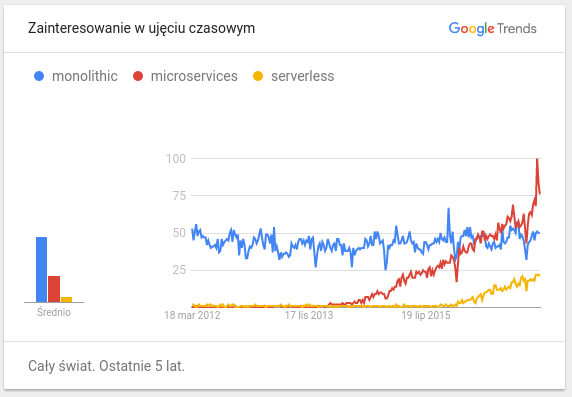
\includegraphics[width=15cm]{2017-03-1321:44:11}
	\caption{Popularność haseł związanych z architekturą aplikacji na przestrzeni ostatnich 5 lat wg Google.}
	\label{fig:popularnoscHaselArchitektury}
\end{figure}

Jak widać na wykresie  \ref{fig:popularnoscHaselArchitektury}, architektura związana z mikroserwisami przewyższa pod względem popularności klasyczną, monolityczną. Jednak nie jest to ostatnie słowo w kwestii migracji architektury w kierunku rozwiązań  dzielących aplikację na mniejsze fragmenty.

Przedstawiona w niniejszej pracy architektura Serverless stanowi raczej ewolucję aniżeli rewolucję w dziedzinie wysokopoziomowego projektu oprogramowania. Zakłada ona podział aplikacji na drobniejsze fragmenty, tj. skalowalnym elementem aplikacji są pojedyncze funkcje, a nie całe serwisy - składające się z funkcji - jak w przypadku architektury mikroserwisowej. Jest to podział bardziej granularny i precyzyjniejszy. Automatyzacja procesu uruchamiania i zamykania kolejnych instancji tych samych funkcji pozwala w locie dostosowywać możliwości obliczeniowe aplikacji jako całości do aktualnego poziomu zapotrzebowania (np. ruchu generowanego przez użytkowników aplikacji). Jak widać na wykresie \ref{fig:popularnoscHaselArchitektury} (strona \pageref{fig:popularnoscHaselArchitektury}), architektura ta powoli zdobywa popularność i zainteresowanie, może się więc okazać najbardziej przyszłościowym rozwiązaniem \cite{kenFrommFutureIsServerless}.

Z teoretycznego punktu widzenia, omawiana architektura posiada więc szereg atutów stawiających ją wyżej od rozpowszechnionej architektury monolitycznej oraz kilka cech pozwalających na konkurowanie z nowoczesną architekturą złożoną z mikroserwisów. Celem niniejszej pracy jest wykazanie wspomnianych we wstępie i wprowadzeniu zalet względem tradycyjnych architektur: atutów takich jak możliwość pozwolenia sobie przez programistów używających Serverless na traktowanie tematyki ściśle serwerowej jako sprawy o drugorzędnym znaczeniu, czy redukcja kosztów spowodowanych używaniem infrastruktury obliczeniowej firm trzecich.

\section{Planowanie przejazdów turystycznych}
Problemy planowania wyjazdu turystycznego wynikają przede wszystkim z różnic tak kulturowych, społecznych jak i ekonomicznych pomiędzy krajami i nacjami. Problemy te dotyczyć mogą bezpośrednio różnic w obowiązującym prawie, zwyczajach społecznych czy chociażby niespodziewanych zmian kosztów podróży tak w jej trakcie, jak i na miejscu. Proponowana aplikacja ma na celu pomóc zaadresować ostatni z wymienionych aspektów - ekonomiczny, a także - częściowo - społeczny.

O rozmiarze problemu ekonomicznego podróżowania świadczyć mogą badania prowadzone przez prywatną firmę Hopper Research, której raport \cite{hopperReseatchFlightTicketPrices} ukazuje średnie fluktuacje cen biletów lotniczych na poziomie od 200 do ponad 1000 dolarów, gdzie kwoty te dotyczą miejsca w tej samej klasie tego samego lotu. Wyszukanie niedrogich biletów lotniczych stanowi więc realny problem związany z kosztami podróżowania. Nie jest to przecież jednak jedyny koszt ponoszony podczas podróży.

Te same fluktuacje dotyczyć mogą także kosztów zakwaterowania w hotelu, pensjonacie, lub - dzięki przybierającym na popularności rozwiązaniom z nurtu sharing-economy \cite{sharingEconomyWhyParticipate} - u prywatnego właściciela mieszkania; a także poruszania się na miejscu docelowym (taksówki, pociągi, inne publiczne środki transportu czy nawet prywatni właściciele pojazdów - ci ostatni znów dzięki sharing-economy \cite{sharingEconomyWhyParticipate}) czy chociażby wyżywienia. Oszczędności płynące ze świadomego podróżowania są zatem realnym przypadkiem użycia dla proponowanej aplikacji.

Wspomnianym problemem społecznym podróżowania jest przepełnienie miejscowości turystycznych w danym czasie, co może znacząco wpływać na komfort odwiedzania nieznanych dotąd miejsc, a także rozdźwięk pomiędzy wyobrażeniem o danym miejscu a jego rzeczywistym stanem \cite{dailyMailTourismExpectationVsReality}, gdzie wyobrażenie kreowane jest między innymi poprzez reklamy czy foldery ofertowe biur turystycznych i podobnych podmiotów, których model biznesowy oparty jest o zachęcanie potencjalnych turystów.

\begin{figure}
	\centering
	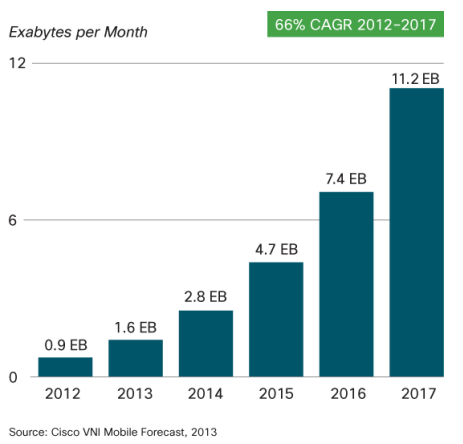
\includegraphics[width=10cm]{2017-03-2018:48:10}
	\caption{Rozmiar ruchu internetowego w eksabajtach / miesiąc i prognoza na rok 2017 wg Cisco \cite{ciscoInternetTrafficSize}}
	\label{fig:rozmiarRuchuWInternecie}
\end{figure}

Adresacja wyżej wymienionych problemów poprzez aplikację webową jest możliwa w oparciu o dane dostępne publicznie poprzez API wybranych firm z sektora prywatnego. Jak widać na wykresie \ref{fig:rozmiarRuchuWInternecie} (strona \pageref{fig:rozmiarRuchuWInternecie}), rozmiar ruchu sieciowego i ilość zbieranych przez firmy trzecie danych o użytkownikach rośnie nieprzerwanie \cite{ciscoInternetTrafficSize}, co skłania do agregacji oraz przetwarzania danych przetaczających się przez Sieć.

Projekt aplikacji zakłada wykorzystanie informacji dostępnych poprzez API takich firm jak Google, Facebook, Uber, Instagram, AirBnB czy Songkick. Problemy ekonomiczne - takie jak nieprzewidywalność kosztów na miejscu czy też fluktuacje cen lotów zaadresowane mogą zostać poprzez wykorzystanie danych z następujących serwisów:
\begin{itemize}
	\item Google QPX Express - API pozwalające wyszukać dostępne loty w dane miejsce
	\item Uber - API pozwalające ocenić koszty transportu w mieście docelowym
	\item AirBnB - API zwraca informacje o potencjalnych miejscach zakwaterowania i umożliwiające dokonanie rezerwacji
	\item Google Maps - API pozwala zebrać informacje o kawiarniach, restauracjach, miejscach kultury jak muzea czy wystawy artystyczne w miejscu docelowym
\end{itemize}


Problemy społeczne natomiast zaadresować można w następujący sposób, wykorzystując publicznie dostępne API:
\begin{itemize}
	\item Google Maps - API pozwalające estymować popularność miejsc w danej chwili
	\item Instagram - API pozwala na pobranie w czasie rzeczywistym zdjęć wykonanych w miejscu docelowym przez turystów lub mieszkańców w tej chwili (ocena rzeczywistego wyglądu miasta / miejsca docelowego)
	\item Facebook Graph API - pobieranie informacji o wydarzeniach w miejscu docelowym, jak koncerty, oraz ocena popularności miejsca na podstawie zameldowań użytkowników w danym miejscu
	\item Songkick API - pobieranie informacji o koncertach w danym miejscu
\end{itemize}

Aplikacja w zamierzeniu nie dokonywałaby wyboru za użytkownika. Model działania docelowo ma być bliższym agregacji i wyświetlaniu danych o potencjalnych miejscach podróży w formie mapy z zaznaczonymi cechami danego miejsca - jak popularność i ocena kosztów całkowitych podróży w zależności od daty podróży oraz strumieniowanym na bieżąco zestawem fotografii z miejsca docelowego. Sam wybór celu podróży pozostawałby w gestii użytkownika. Poprzez wyświetlenie użytkownikowi estymacji kosztów podróży w danym terminie w dane miejsce, za pomocą atrakcyjnej wizualnie mapy, aplikacja stanowić będzie nieocenioną pomoc w kwestii wyboru celu, wliczając nie tylko same koszty logistyczne, ale też koszty związane z wydarzeniami na miejscu.

\section{Architektura Serverless}
Samo pojęcie Serverless zostało po raz pierwszy użyte w publikacji autorstwa Kena Fromma w roku 2012 w artykule "Why The Future Of Software And Apps Is Serverless". Jak podkreślał autor, nomenklatura jest nieco myląca - pojęcie Serverless nie oznacza, że w systemie komputerowym nie ma serwera w sensie fizycznej maszyny \cite{kenFrommFutureIsServerless}, a raczej o fakt, że zaproponowanym podejściu, w procesie rozwijania oprogramowania programiści nie muszą myśleć o zasobach sprzętowych (serwerach) i ich administracji, natomiast powinni skupić się na samej domenie biznesowej i wyodrębnieniu pojedynczych zadań, które wykonuje aplikacja.

W zaproponowanym podejściu, odpowiedzialność za wdrożenie, uruchomienie oraz skalowanie aplikacji spoczywa na wybranym dostawcy usługi chmurowej. Jest to więc swojego rodzaju outsourcing całego problemu związanego z administracją tworzonej aplikacji - rolą programisty pozostaje dostarczenie samego kodu i umieszczenie go na platformie dostarczonej przez dostawcę.

W podejściu Serverless, jednostka wykonawcza to zazwyczaj pojedyncza funkcja programu. Programiści mający doświadczenie z aplikacjami opartymi o mikroserwisy kojarzyć mogą pojedynczą funkcję z endpointem pojedynczego API. Warunkiem działania aplikacji jest oczywiście bezstanowość tychże pojedynczych funkcji, z których aplikacja się składa. Dzięki bezstanowości, dostawcy usług na życzenie uruchamiają kolejne instancje (replikują) dostarczonej funkcji - co pozwala reagować na zmiany w sposobie użytkowania programu, głównie dlatego, że uruchamianie kolejnych instancji funkcji może być w pełni zautomatyzowane i dostosowane do obciążenia zadaniami. Wraz z rosnącą popularnością, programiści nie muszą planować wydajności maszyny zakładając margines błędu i potencjalną liczbę użytkowników ani obawiać się limitu wydajności platformy na jakiej uruchomili aplikację.

Wśród dostawców platform opartych o architekturę Serverless prym wiedzie zaprezentowana w 2014 roku platforma AWS Lambda, wśród usług wartych wymienienia sa również OpenWhisk (opracowany przez IBM), frameworki Funktion oraz LeverOS (oparte o system kontenerów), oraz IronWorker.

\subsection{Definicja architektury Serverless}
Definicji architektury Serverless podjął się Mike Roberts w artykule opublikowanym na blogu MartinFowler.com \cite{martinFowlerServerless}. Przede wszystkim zauważył on, iz pojęcie Serverless używane jest do opisu dwóch, niekoniecznie powiązanych zjawisk dotyczących projektowania aplikacji.

\begin{figure}
	\centering
	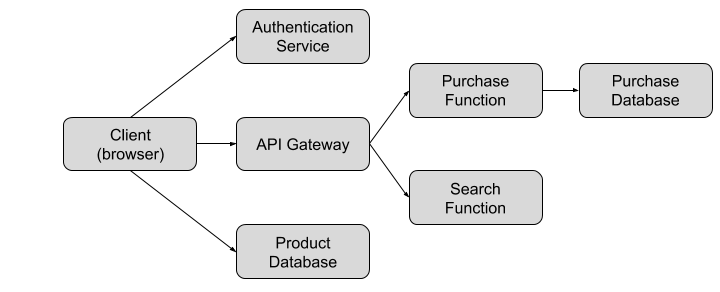
\includegraphics[width=15cm]{2017-04-1010:44:19}
	\caption{Architektura przykładowej aplikacji opartej na Backend as a Service \cite{martinFowlerServerless}}
	\label{fig:schematArchitekturyBaaS}
\end{figure}


Pierwszym z nich jest architektura polegająca na wykorzystywaniu zewnętrznych, często publicznych usług, które rozwiązują powszechnie spotykane problemy napotykane podczas prac nad aplikacją webową. Przykładem takiego problemu jest zarządzanie kontami użytkowników czy też proces logowania użytkowników, lub cała warstwa persystencji aplikacji. Taki typ architektury został przez Robertsa nazwany "BaaS" (Backend as a Service) \cite{martinFowlerServerless}. Zastąpienie własnej implementacji usługą dostarczoną przez zewnętrznego usługodawcę (jako przykład podać można OAuth w przypadku logowania użytkowników lub Firebase, będący usługą dostarczającą bazę danych) niweluje czas potrzebny na rozwój aplikacji, jednak zmusza do pewnych ustępstw w kwestii dopasowania usługi do specyfiki aplikacji - korzystając z zewnętrznego serwisu, niemożliwa jest oczywiście edycja kodu lub zmiana funkcjonalności takiej usługi.

\begin{figure}
	\centering
	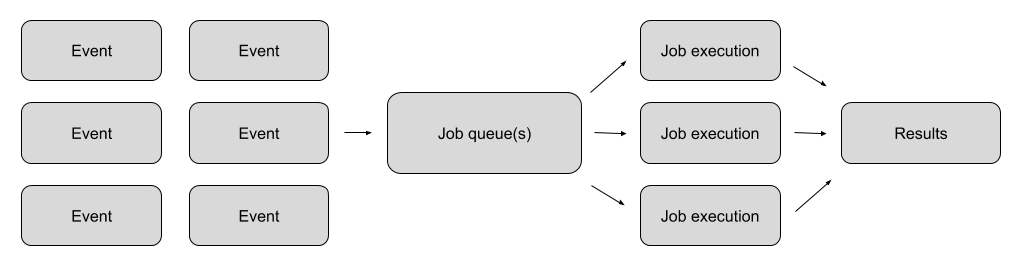
\includegraphics[width=15cm]{1-Qv681cjXguRg-H1XyLcxXw}
	\caption{Schemat przetwarzania zadań w Function as a Service \cite{kenFrommThinkingServerless}}
	\label{fig:schematDzialaniaFaaS}
\end{figure}

Drugim konceptem architektury aplikacji, do opisu którego wykorzystuje się pojęcie Serverless, jest tak zwana architektura FaaS (Function as a Service) \cite{martinFowlerServerless}. Idąc za Robertsem, przykładem zastosowania architektury FaaS jest aplikacja, w której część logiki wykonywana jest na maszynach obliczeniowych dostarczanych i zarządzanych przez firmy trzecie. W takim wypadku, logika aplikacji jest tworzona całkowicie przez programistę, natomiast za samo wykonanie kodu odpowiadają zazwyczaj kontenery tworzone i działające na serwerach firmy zewnętrznej.


Bardziej aktualnym dla określenia Serverless jest właśnie drugi koncept - FaaS, wedle którego działa największy dostawca tego typu usług, AWS Lambda. Roberts podkreśla, że w tym podejściu traci na znaczeniu zarządzanie serwerem czy też systemem serwerów; zastosowanie architektury FaaS pozwala również wyeliminować potrzebę posiadania zawsze dostępnego serwera obliczeniowego, który uruchomiony jest bez względu na wykorzystanie aplikacji.

Dzieje się tak ponieważ kontenery uruchamiane przez usługodawcę reagują na wydarzenie - którego wyzwolicielem może być czas (działaniem przypominają wtedy programy związane z harmonogramami, np. \textit{cron}), pojawienie się lub zmiana zawartości publicznie dostępnego pliku, bądź pojawienie się wiadomości na kolejce - i uruchamiane są tylko w razie potrzeby (pojawienie się zadania do wykonania), a ich czas życia ogranicza się tylko do tego właśnie zadania, co zilustrowane jest na schemacie \ref{fig:schematDzialaniaFaaS} (strona \pageref{fig:schematDzialaniaFaaS}). Po jego wykonaniu zostają usunięte, a w razie potrzeby usługodawca tworzy kolejne kontenery wykonujące nadchodzące zadania. Taki charakter działania kontenerów określa się mianem ulotnego (z ang. \textit{ephemeral}, tłum. własne).

\begin{figure}
	\centering
	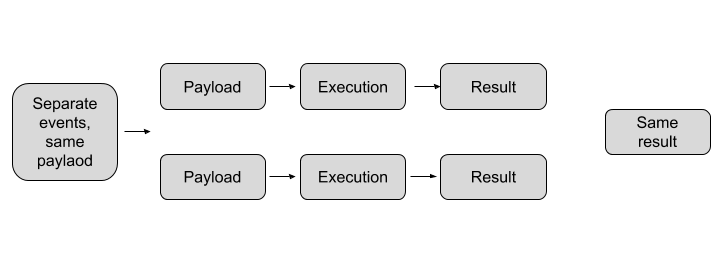
\includegraphics[width=15cm]{0-zJwqKxUVXdMjDboR}
	\caption{Idempotentność zadań w podejściu Function as a Service \cite{kenFrommThinkingServerless}}
	\label{fig:idempotentnoscFaaS}
\end{figure}

Jak zostało powiedziane wcześniej, funkcja działająca w kontenerze jest całkowicie bezstanowa, co zapewnia jej idempotentność wykonywania zadań (na schemacie \ref{fig:schematDzialaniaFaaS}, strona \pageref{fig:schematDzialaniaFaaS}). Implikuje to możliwość nieograniczonego skalowania kontenera zawierającego taką funkcję w zależności od potencjalnego obciążenia systemu. To z kolei zapewnia programiście transparentne skalowanie się aplikacji, które w dodatku zachodzi bez jego udziału - w przypadku nadejścia wzmożonego ruchu (i, co za tym idzie, większej ilości zadań na kolejce), usługodawca samodzielnie uruchamia więcej kontenerów ze zdefiniowaną przez programistę funkcją, pozwalając na nieprzerwane i wydajne działanie systemu.

\subsection{Porównanie z alternatywnymi architekturami}
By uwypuklić cechy szczególne prezentowanego w pracy podejścia do projektowania aplikacji, do porównania wybrane zostały dwie starsze, cieszące się ugruntowaną popularnością architektury: klasyczna Model-View-Controller (MVC) oraz nowocześniejsza, zorientowana na wydarzenia (z ang. events) architektura wykorzystująca bibliotekę umożliwiającą obliczenia współbieżne.

O ile wybór pierwszej, kanonicznej architektury podyktowany jest względami teoretycznymi, tj. wykazanie istnienia różnic w charakterze pracy z wymienionymi architekturami oraz wypunktowanie ich możliwości, o tyle ciekawsze wydaje się być porównanie praktyczne z architekturą opartą o obliczenia rozproszone, w której aplikacja działa w kontenerach uruchamianych na własnym, lokalnym serwerze.

\begin{figure}
	\centering
	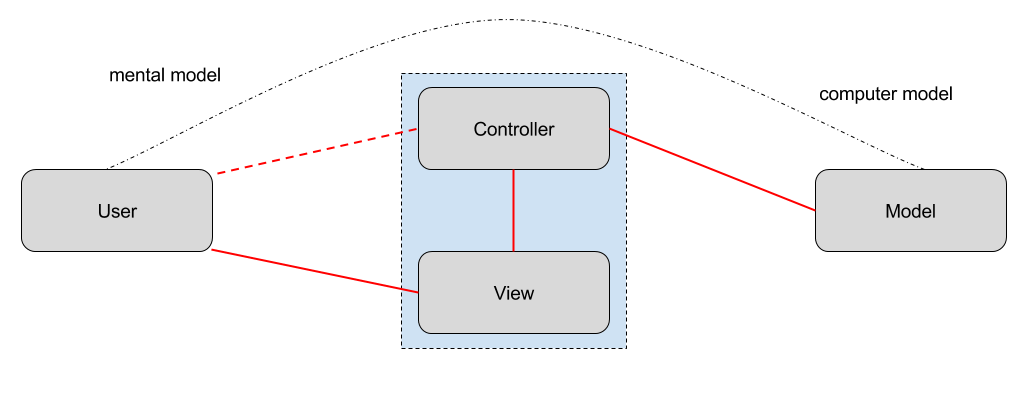
\includegraphics[width=15cm]{artima-mvcu}
	\caption{Szkic przełożenia logiki biznesowej na wyobrażenie o nim użytkownika za pomocą architektury MVC  \cite{artimaDciArchitecture}}
	\label{fig:mentalModelMvc}
\end{figure}

\subsubsection{Architektura MVC}
Klasyczna architektura MVC zaproponowana została w późnych latach 80. W założeniach, jest to architektura powstała z myślą o aplikacjach wyposażonych w interfejs użytkownika i mająca za zadanie ułatwić przełożenie zaprojektowanego przez programistę \textit{Modelu} (dowolnego bytu - \textit{encji} bądź klasy wykonującej jakąś czynność związaną z domeną biznesową, tzw. \textit{logikę biznesową}) na wyobrażenie (tzw. \textit{mental model}) o tymże modelu u użytkownika \cite{artimaDciArchitecture}, co pokazuje ilustracja \ref{fig:mentalModelMvc}. (strona \pageref{fig:mentalModelMvc}).

Kolejnym elementem architektury MVC jest Widok (\textit{View}). Reprezentuje on pewną perspektywę na wspomniany Model, specyficzną dla danego użytkownika aplikacji. W dużym uproszczeniu jest to zbiór wybranych informacji o modelu (w szczególnym przypadku będącym encją) przedstawionych poprzez interfejs graficzny użytkownikowi aplikacji \cite{artimaDciArchitecture}. Przykładowym Modelem może być zbiór informacji kontaktowych osoby fizycznej, a Widokiem - wycinek tychże informacji, potrzebny użytkownikowi aplikacji - dajmy na to, telemarketerowi - któremu do pracy potrzebny jest jedynie numer telefonu. W aplikacji webowej pojęcie Widoku dotyczyć może również danych łącznie z wizualizacją, np. witryną internetową prezentującą te dane.

Ostatnim elementem architektury jest Kontroler (\textit{Controller}), zapewniający przepływność danych pomiędzy Modelem a Widokiem i koordynujący działania aplikacji, np. interpretując akcje użytkownika, generując Widoki i zwracając je do niego \cite{artimaDciArchitecture}. Na schemacie przepływu danych pomiędzy elementami architektury MVC (\ref{fig:mentalModelMvc}, strona \pageref{fig:mentalModelMvc}) zauważyć można podział odpowiedzialności poszczególnych komponentów.

\begin{figure}
	\centering
	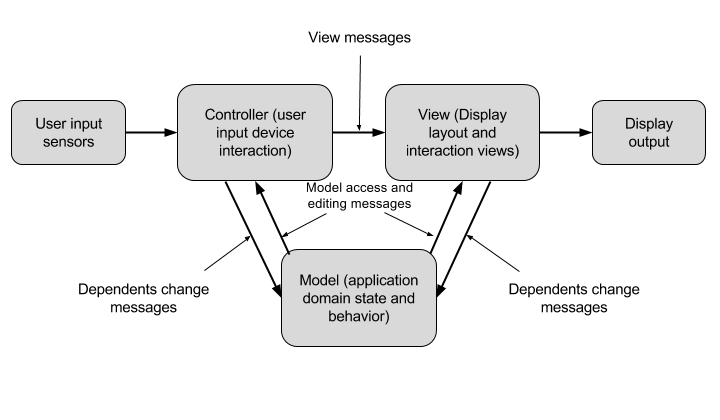
\includegraphics[width=15cm]{mvc-scheme}
	\caption{Architektura Model - View - Controller \cite{krasnerPopeMvcUiParadigm}}
	\label{fig:mvcArchitecture}
\end{figure}

Porównanie zaproponowanej w niniejszej pracy architektury Serverless z klasyczną MVC w kontekście aplikacji webowej sprowadzać musi się do teoretycznego wypisania cech ułatwiających i utrudniających rozwój aplikacji osadzonej w pierwszej bądź drugiej architekturze. W przypadku współczesnych implementacji MVC, jak na przykład ASP.NET MVC, niewątpliwym plusem jest szybkość rozwoju aplikacji opartej na tej architekturze - za pomocą podążania za pewnymi schematami podsuwanymi przez wzorzec zaproponowany przez Microsoft, większość typowych problemów jest rozwiązywana za programistę, co pozwala skupić się bezpośrednio na implementacji logiki biznesowej w Modelach. Przykładami gotowych rozwiązań mogą być: projekty reprezentacji Widoków w formie witryny WWW, internacjonalizacja całej aplikacji, gotowe rozwiązania do autoryzacji użytkowników czy rozwiązywanie adresów URL Kontrolerów.

Minusów podejścia opartego o MVC jest jednak więcej. Między innymi są to konieczność użycia jednego, wybranego frameworka (który udostępni nam wachlarz gotowych rozwiązań typowych problemów), a co za tym idzie - jednego języka programowania do całości aplikacji, co może stanowić problem w przypadku kompleksowego projektu. Natomiast w podejściu Serverless nie stanowi to problemu dzięki zunifikowanemu modelu komunikacji opartego o API (zazwyczaj HTTP, np. REST API), co umożliwia implementację poszczególnych serwisów w dowolnych technologiach. Kolejnym z minusów jest brak wpisanej w tożsamość architektury skalowalności - we współczesnych implementacjach MVC większość obciążenia skupia się na Kontrolerach, które - domyślnie - nie skalują się horyzontalnie. Jest to oczywiście możliwe do obejścia za pomocą własnych rozwiązań - np. rozpisanie kontrolerów na wiele serwerów poprzez rozbicie czynności na osobne API. Jest to jednak pewnego rodzaju proteza dopisana do architektury, której - w zamyśle - nie należało rozszerzać o takie funkcjonalności, i po zastosowaniu takowej protezy, przypominać zaczyna nowoczesne API, jak SOAP czy REST.

Dla kontrastu, w architekturze Serverless najbardziej zbliżony funkcjonalnością Kontrolerowi z MVC komponent, czyli API Gateway (widoczny na schemacie \ref{fig:schematArchitekturyBaaS}, strona \pageref{fig:schematArchitekturyBaaS}) jest mniej obciążony, ponieważ jego jedyną funkcjonalnością jest przesyłanie żądań do odpowiednich funkcji na serwerach firm trzecich. W razie jednak potrzeby zeskalowania także tego komponentu, nie stanowić to powinno problemu z uwagi na fakt, że Gateway jest zwykłym API (np. REST), nic nie stoi więc na przeszkodzie, by takie API uruchomić na kilku niezależnych maszynach i dodać do architektury warstwę pośredniczącą, która zapewni rozłożenie obciążenia pomiędzy maszyny z uruchomionym komponentem Gateway (Load Balancing).

\subsubsection{Architektura rozproszona}
Ciekawszym przypadkiem porównawczym jest zestawienie Serverless z rozwiązaniem również zorientowanym na obliczenia współbieżne oraz umożliwiającym skalowanie horyzontalne, ale w nieco bardziej klasycznej formie. Takie porównanie nie może jednak składać się jedynie z teoretycznego zestawienia ze sobą cech z uwagi na podobieństwo działania - zmienia się jedynie ziarnistość jednostki skalowanej (funkcja w Serverless kontra aplikacja / klient w mikroserwisie) i wykorzystane biblioteki.

W zaproponowanym podejściu, klienci żądający wyników, wysyłają swoje żądania do centralnego elementu będącego kolejką zadań. Element zwany brokerem zapewnia rozłożenie żądań na pewną liczbę wykonawców, realizujących żądania. Odbiór wyników może się różnić w zależności od implementacji. Schemat działania takiej architektury pokazuje ilustracja \ref{fig:ClassicDistributedArch}.

\begin{figure}
	\centering
	\includegraphics[width=16cm]{ClassicDistributedArch}
	\caption{Schemat przesyłu komunikatów w zaproponowanej do porównania architekturze rozproszonej}
	\label{fig:ClassicDistributedArch}
\end{figure} 

Aplikacja rozproszona zastosowana do porównania oparta będzie więc na tym samym języku, ale wykonana z wykorzystaniem biblioteki Celery. Punktem wspólnym dla obu przypadków jest fakt zorientowania na wydarzenia (events) i zadania (tasks) oraz istnienie tzw. API Gateway, które stanowi warstwę pośrednią pomiędzy front-endem oraz kolejkami zadań obsługiwanymi przez Celery (w Serverless API Gateway odpowiadało za przekierowania żądań na odpowiednie funkcje). Schemat przepływu danych pomiędzy komponentami w tej architekturze opisuje ilustracja \ref{fig:PracaInzCeleryArchitecture} (strona \pageref{fig:PracaInzCeleryArchitecture}).

\begin{figure}
	\centering
	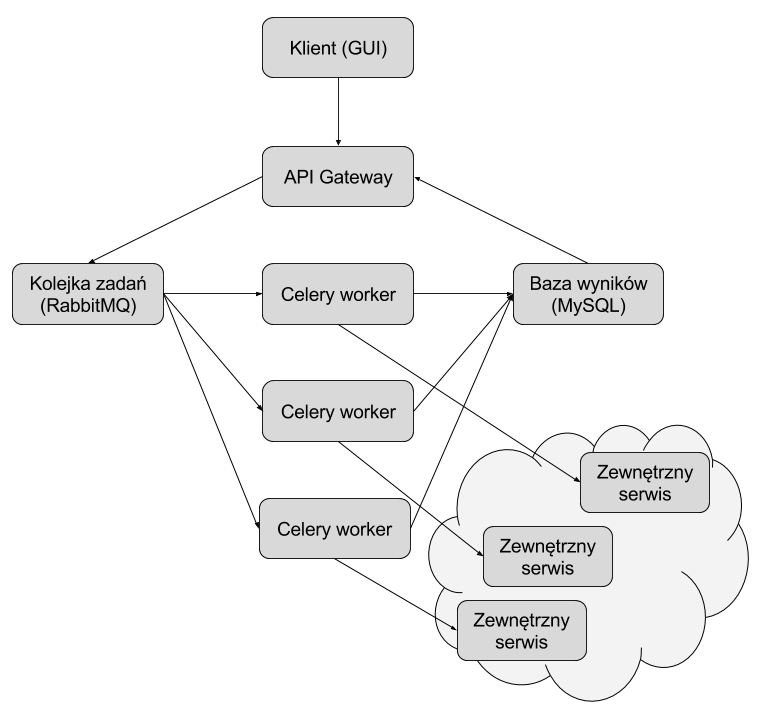
\includegraphics[width=15cm]{PracaInz-CeleryArchitecture}
	\caption{Architektura aplikacji porównawczej opartej o Celery}
	\label{fig:PracaInzCeleryArchitecture}
\end{figure}

W działania aplikacji wykonanej w architekturze klasycznej wymagane są dwa dodatkowe komponenty - serwer wiadomości implementujący interfejs AMQP (wybrany został RabbitMQ jako najpopularniejszy i rekomendowany dla biblioteki Celery), który działa również jako broker wiadomości (element rozsyłający wiadomości - tu zadania - do odpowiednich procesów wykonawczych; RabbitMQ stosuje strategię round robin), oraz tzw. backend - usługę zapewniającą trwałość wyników zadań (persistency). Pomimo że rekomendowanym rozwiązaniem dla tego zastosowania jest Redis, będący nierelacyjną bazą danych trzymaną w pamięci, nie udało się zmusić do komunikacji biblioteki Celery i tejże bazy - okazuje się, że ze względu na niedojrzałość biblioteki Celery, ma ona szereg problemów komunikacyjnych - problem zaraportowany 9. marca w obrębie serwisu github.com na funkcję komunikacji z tą bazą pozostaje otwarty (numer: 3898) do dnia dzisiejszego (czerwiec). Jako działająca alternatywa, wybrany został serwer relacyjnej bazy danych MySQL, z którym komunikacja okazała się bezproblemowa. 

Obie aplikacje różnić się będą sposobem uruchamiania i wdrażania. O ile ten problem praktycznie nie istnieje w przypadku Serverless, o tyle w architekturze klasycznej, kolejne serwisy zamykane będą w kontenerach (wybrany został Docker jako najpopularniejsze obecnie rozwiązanie) i uruchamiane niezależnie na tej samej bądź różnych maszynach wirtualnych, co pozwoli między innymi na skalowanie horyzontalne. Oba komponenty wspomniane wyżej w kontekście architektury rozproszonej klasycznej, tj. serwer wiadomości oraz serwer wyników - zostały uruchomione za pomocą kontenerów, by uniknąć czasochłonnych instalacji i konfiguracji przy każdym testowym uruchomieniu aplikacji.

Głównym celem porównania jest odpowiedź na pytanie: czy Serverless jest bardziej opłacalny jeśli chodzi o łatwość rozwoju oprogramowania, wdrożenie oraz wydajność względem klasycznej architektury rozproszonej? Miarą opłacalności będzie subiektywna trudność implementacji serwisów w jednym i drugim podejściu, trudność ich uruchamiania  oraz wydajność infrastruktury przy danym obciążeniu, gdzie przez wydajność rozumiany jest czas realizacji żądań wysłanych do API. W teorii, aplikacja wykonana w Serverless powinna być prostsza w implementacji oraz lepiej skalowalna i łatwiejsza w utrzymaniu (gdyż nie ma potrzeby uruchamiać dodatkowych serwerów w przypadku lawinowego obciążenia). W praktyce jednak okazać się może, że usługi typu Serverless są nadal zbyt świeże, co spowoduje trudności w implementacji, ponieważ Serverless nie dysponuje jeszcze tak dobrym wsparciem społeczności.

\chapter{Projekt aplikacji w architekturze Serverless}
\begin{figure}
	\centering
	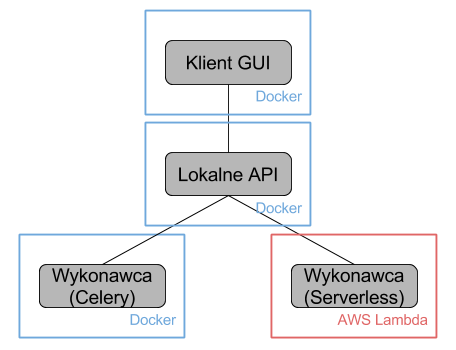
\includegraphics[width=13cm]{app_architecture}
	\caption{Główne komponenty opracowanej aplikacji}
	\label{fig:AppComponents}
\end{figure}

Aplikacja opracowana na potrzeby pracy składa się z 3 głównych komponentów: interfejsu użytkownika zbudowanego za pomocą frameworka Angular.js, lokalnego komponentu API Gateway w postaci Web Service zbudowanego z użyciem klasycznego serwera WWW CherryPy, który - za pomocą klasy czerpiącej z wzorca Serwisu - przekierowuje żądania na konkretne zadania i przekazuje je do ostatniego komponentu - wykonawcy, zaimplementowanego w dwóch wersjach. Pierwszą wersją jest wspomniany wyżej framework Celery, wspomagający wykonywanie rozproszone, drugą natomiast wersją jest środowisko dostarczane przez AWS (usługa Lambda, wspomniana wcześniej w pracy), do którego wysyłane są żądania. Schemat podziału aplikacji na komponenty widnieje na ilustracji \ref{fig:AppComponents} (strona \pageref{fig:AppComponents}).

Jak widać na schemacie, komponenty uruchamiane są w izolowanych kontenerach opartych na implementacji Docker, jedynie wykonawca zdalny - dostarczany przez AWS - działa w nie określonym środowisku, a komunikacja doń odbywa się poprzez Internet. AWS jako usługodawca dostarcza również zdalne API Gateway, które zajmuje się wysyłaniem wydarzeń do kontenerów z funkcjami. Wynika więc z tego, że w wersji z wykonawcą opartym o usługę Lambda, żądanie przechodzi przez dwa API Gateway - lokalne, działające w kontenerze Dockerowym, oraz zdalne, uruchomione na serwerze AWS. W obu API ruch odbywa się poprzez protokół HTTP, a dane przesyłane są w formacie JSON. Schemat \ref{fig:AppLambdaCommunicationsScheme} na stronie \pageref{fig:AppLambdaCommunicationsScheme} ilustruje komunikację między lokalnym a zewnętrznym API.

\begin{figure}
	\centering
	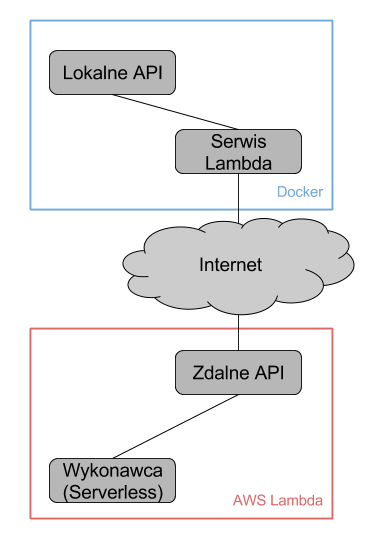
\includegraphics[width=9cm]{app_lambda_architecture}
	\caption{Schemat przesyłania komunikatu z użyciem AWS Lambda}
	\label{fig:AppLambdaCommunicationsScheme}
\end{figure}

Komunikacja na poziomie lokalnego API jest synchroniczna, tj. pojedyncze żądanie wysłane do API trwa, dopóki nie zwróci wyniku realizacji zadania (kod HTTP 200 sygnalizuje pomyślnie wykonane zadanie). Asynchroniczność w działaniu aplikacji zapewnia komponent stanowiący interfejs użytkownika - żądania wysyłane przezeń (angularjs) do końcówek (z ang. endpoint) API nie powodują przeładowania aplikacji, użytkownik nie jest więc świadom synchroniczności komunikacji (zapewniona jest tym samym przezroczystość wykonania). Serwer WWW na którym opiera się lokalne API Gateway skonfigurowany jest tak, by działać jednocześnie na wielu wątkach, co zapewnia obsługę wielu żądań, synchroniczność pojedynczych połączeń na poziomie lokalnego API nie przeszkadza więc w obsłudze wielu użytkowników.

Do obsługi usługi AWS Lambda wybrany został najpopularniejszy - w czasie pisania pracy - framework stworzony w tym celu, Serverless Framework. Zapewnia on zarządzanie zależnościami danej funkcji, jej pakowanie, przesyłanie i wdrażanie w zdalnym środowisku AWS. Framework ten nadal jest w fazie beta i miewa problemy z niektórymi zadaniami, jednak najważniejsza funkcjonalność okazała się działać bez zarzutu. Jedyny przypadek z którym pojawiły się problemy to zależności do lokalnego modułu zawierającego kod, na którym polega pakowana do usługi funkcja - Serverless Framework nie wspiera instalacji zależności wewnątrz modułu w trybie edytowalnym - przy każdej aktualizacji kodu zdalnego konieczna była ponowna instalacja pakietów, do których zależności miała funkcja.

Interfejs graficzny użytkownika został oparty na połączeniu angularjs, która zapewnia komunikację między renderowaną zawartością a danymi dostarczanymi przez API oraz technologii Bootstrap, zapewniającej automatyczne skalowanie interfejsu aplikacji do urządzenia użytkownika. Jak pokazują ilustracje, interfejs zmienia rozmieszczenie poszczególnych elementów w zależności od szerokości wyświetlacza urządzenia, z którego korzysta użytkownik - ilustracja \ref{fig:guiBootstrapPC} ukazuje rozmieszczenie elementów wyników żądań na ekranie o rozdzielczości w standardzie FullHD, układ zaprezentowany na ilustracji \ref{fig:guiBootstrapTablet} - rozmieszczenie na ekranie urządzenia typu tablet, a ilustracja \ref{fig:guiBootstrapPC} - układ elementów na ekranie urządzenia mobilnego, np. smartfona.

\begin{figure}
	\centering
	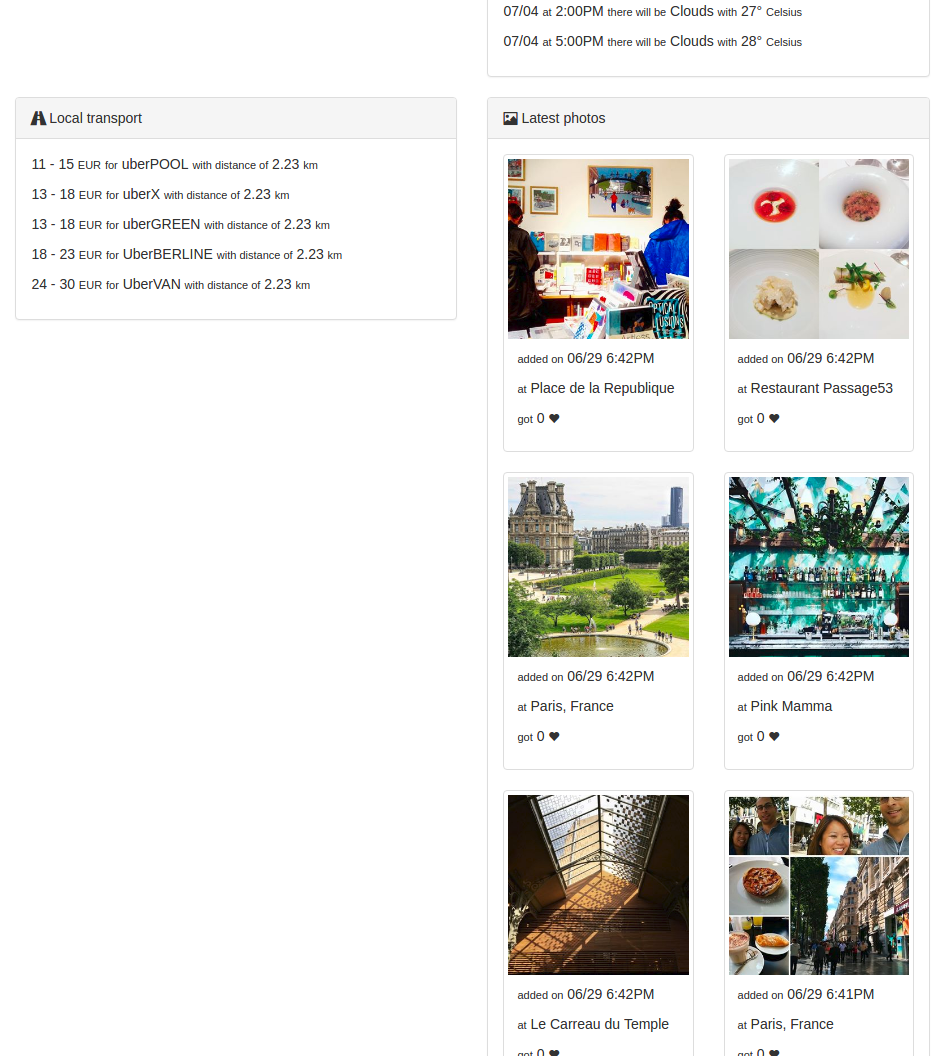
\includegraphics[width=11.5cm]{2017-06-2918:42:27}
	\caption{Rozmieszczenie elementów interfejsu graficznego na ekranie tabletu}
	\label{fig:guiBootstrapTablet}
\end{figure}

\begin{figure}
	\centering
	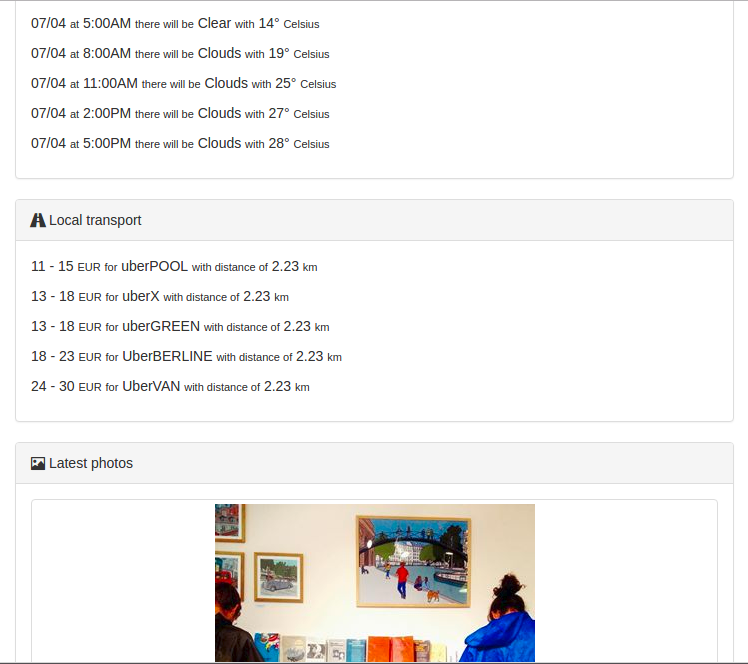
\includegraphics[width=8cm]{2017-06-2918:52:04}
	\caption{Interfejs graficzny na ekranie smartfona}
	\label{fig:guiBootstrapSmartphone}
\end{figure}

\begin{figure}
	\centering
	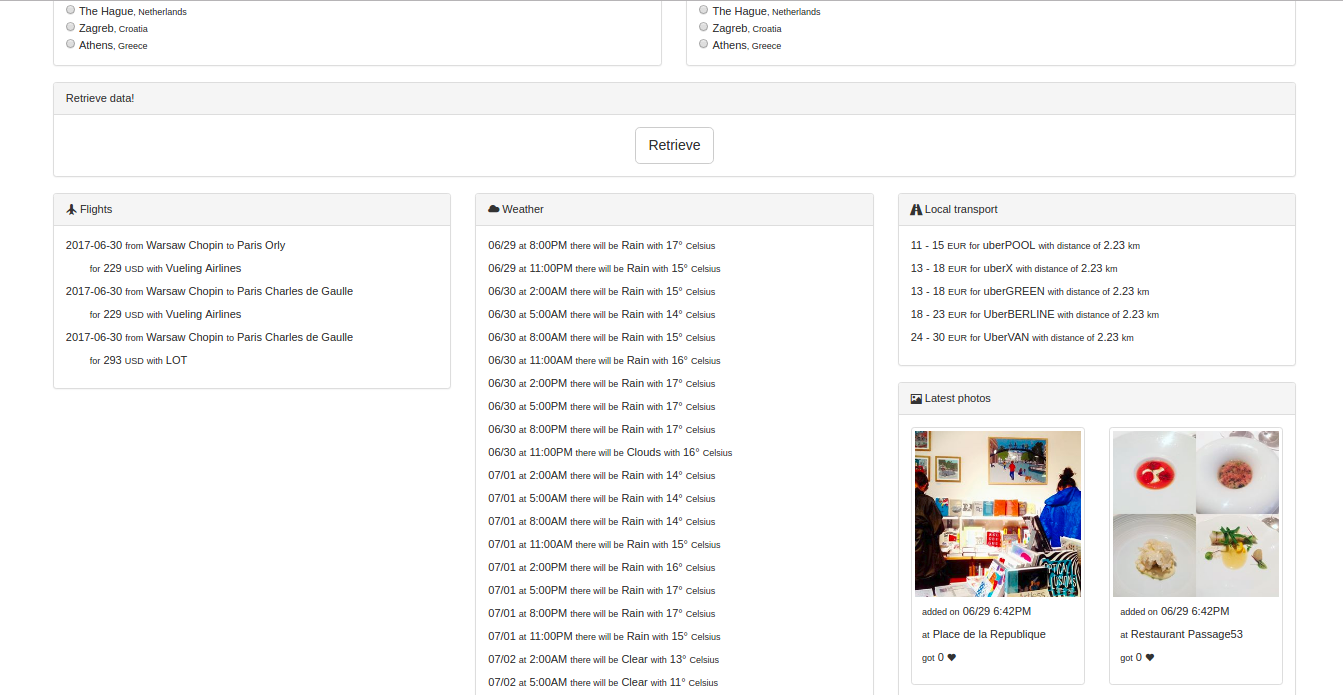
\includegraphics[width=15cm]{2017-06-2918:53:18}
	\caption{Interfejs graficzny na ekranie komputera}
	\label{fig:guiBootstrapPC}
\end{figure}

Uzupełnianie implementacji wspomagane było również przez testy jednostkowe. Przypadki testowe pokrywały w głównej mierze metody konwertujące dane pochodzące z firm trzecich i przekładające je na wewnętrzne reprezentacje (modele), używane przez pisaną aplikację. Testy zapewniały więc kontrakt pomiędzy API firm trzecich a komunikacją wewnętrzną aplikacji wykonanej na potrzeby niniejszej pracy inżynierskiej. Pakiet testów uruchamiany był za pośrednictwem usługi Travis CI przynajmniej raz dziennie, a także przy każdej zmianie kodu - usługa Travis zsynchronizowana była ze zdalnym repozytorium kodu znajdującym się na serwerze serwisu github.com.

Podczas rozwoju aplikacji zaistniał problem dzielenia wspólnego kodu pomiędzy obrazami kontenerów - został on rozwiązany poprzez dziedziczenie obrazów kontenerów. Mechanizm ten polega na wywodzeniu się obrazu z innego (klauzula FROM w pliku definiującym obraz, czyli Dockerfile w przypadku Dockera). Utworzony został więc obraz zawierający wspólne części kodu, bazujący na dystrybucji Linuxa Debian 8, i z niego wywodzą się odpowiednio obrazy dla Gateway API, GUI oraz Wykonawcy. Moduł odpowiedzialny za wywołanie funkcji na zdalnej usłudze Lambda nie jest uruchomiony jako niezależna aplikacja, nie ma więc swojego obrazu kontenera.

\chapter{Badanie wydajności aplikacji}
Badanie wydajności w przypadku obu proponowanych architektur polegało na dwóch scenariuszach testowych uruchomionych dla każdej z implementacji. Oba scenariusze polegały na symulacji wysłania pewnej ustalonej liczby zapytań o zasoby jednocześnie do lokalnego API Gateway.

W przypadku architektury rozproszonej klasycznej, opartej na Celery, API Gateway przesyłało żądanie do zadania realizowanego w lokalnej maszynie testowej na wielu niezależnych procesach, która realizowała żądanie do zewnętrznego API firmy trzeciej i zwracała wynik do lokalnego API Gateway (pośrednio poprzez serwer bazy danych MySQL). Zadanie pobrania wyniku z serwisu zewnętrznego nie należy do kategorii zadań obciążających procesor, nie stanowił więc on wąskiego gardła w eksperymencie.

Architektura oparta o AWS Lambda składała się z dodatkowego żądania HTTP: żądanie ze skryptu testującego wydajność trafiało do lokalnego API Gateway; stamtąd przekierowane było - również jako żądanie HTTP - do serwera firmy Amazon, do tzw. zdalnego API Gateway, które uruchamiało funkcję umieszczoną w usłudze Lambda, która z kolei realizowała właściwe żądanie do serwera firmy trzeciej. Spodziewany był więc wyraźnie słabszy wynik ze strony architektury Serverless.

Scenariusze weryfikowały zdolność skalowalności, tzn. scenariusz pierwszy zakładał ruch mieszczący się w konfiguracji przewidzianej przy wdrożeniu aplikacji opartej na Celery, drugi - przekraczał założone wartości i miał pokazać spadek wydajności przy zbyt obciążonych serwerach. W pierwszym przypadku, ruch generowany był przez 16 "użytkowników", z których każdy wysyłał po 4 żądania do każdego z czterech lokalnych końcówek Gateway API, co wygenerowało 256 żądań podczas całego scenariusza. W drugim przypadku użytkowników jednocześnie korzystających z serwisu było już 32, co dało wynik 512 żądań. Testy przeprowadzane były na realnych API firm trzecich, co znacząco wpłynęło na ograniczenie rozmiaru testów - darmowy dostęp do niektórych z tych API zakładał dzienny limit rzędu 1000 żądań, stąd niewielki rozmiar próby testowej.

Wdrożenie obu implementacji zakładało uruchomienie lokalnego API zdolnego do przetworzenia 32 żądań jednocześnie (ustawienie dla CherryPy, serwera WWW na którym oparte zostało lokalne API Gateway), a liczba procesów-wykonawców we frameworku Celery została ograniczona do 16, co oznaczało, że siedemnaste żądanie zostawało umieszczone w kolejce, co spowalniało odpowiedź z API. Scenariusz pierwszy zakładał więc całkowite wykorzystywanie zasobów Wykonawcy w przypadku implementacji opartej o Celery, drugi zaś - przekroczenie tej liczby, a więc symulacja lawinowego ruchu. Ograniczenie to nie dotyczyło implementacji opartej o AWS Lambda - funkcje miały o wiele wyższy limit replikacji (i tym samym zdolność do obsługi większej ilości zapytań jednocześnie), co odzwierciedla niewrażliwość na niedoszacowaną konfigurację podczas wdrożenia.

\begin{table}[t]
	\begin{tabular}{|l|l|r|r|r|r|}
		\hline 
		Scenariusz & Implementacja & Minimalny & Maksymalny & Średni & Mediana\\
		\hline
		1. & Celery & 0,54 & 5.85 & 1,42 & 1,17 \\
		\hline
		1. & AWS Lambda & 0,19 & 5,32 & 1,41 & 1,10 \\
		\hline
		2. & Celery & 1,39 & 9,66 & 3,41 & 3,19 \\
		\hline
		2. & AWS Lambda & 0,78 & 7,27 & 2,59 & 1,90 \\
		\hline
	\end{tabular} 
	\caption{Wyniki testów wydajnościowych - czasy odpowiedzi (w sekundach)}
	\label{perfResultsTable}
\end{table}

Pierwszym ciekawym wnioskiem wynikającym z wyników zawartych w tabeli testów wydajności jest fakt, że dodatkowe żądanie HTTP pojawiające się w trakcje realizacji każdego z żądań testowych w architekturze opartej na usłudze AWS Lambda miało marginalny wpływ na wynik testu wydajności. Średnia i mediana dla obu implementacji w przypadku pierwszego scenariusza są zbliżone, co sugeruje istnienie połączenia o bardzo niskiej latencji pomiędzy serwerami usługi Lambda a serwerami API firm trzecich. Również połączenie pomiędzy maszyną testową (lokalnym serwerem) a serwerem usługi Lambda (zlokalizowanym we Frankfurcie) musi być zatem nieco szybsze niż bezpośrednie połączenie do API firm trzecich.

Drugim, kluczowym dla pracy wnioskiem jest konfrontacja wyników scenariusza drugiego, zakładającego przekroczenie zakładanej liczby użytkowników, wynikającego z niedoszacowania obciążenia serwera utrzymującego aplikację. W tym przypadku potwierdziły się atuty architektury opartej o rozwiązanie Serverless - kolejkowanie żądań wysłanych do implementacji opartej o bibliotekę Celery podczas gdy wszystkie procesy były zajęte zaowocowało ogromnym wydłużeniem średniego czasu wykonania żądania (240\% oryginalnego czasu oczekiwania dla średniej, 273\% dla mediany). Problem ten dotknął też architekturę Serverless, ale w znacznie mniejszym stopniu (180\% oryginalnego czasu oczekiwania dla średniej, 172\% dla mediany).

Wyniki badań wydajności potwierdzają popularną tezę mówiącą, że architektura oparta o zewnętrzne funkcje zapewnia lepszą skalowalność, szczególnie w przypadkach przekroczenia zakładanego obciążenia serwera.

\chapter{Podsumowanie}
Oryginalny problem postawiony we wstępie niniejszej pracy brzmi: czy Serverless jest bardziej opłacalny jeśli chodzi o łatwość rozwoju oprogramowania, wdrożenie oraz wydajność względem klasycznej architektury rozproszonej? Podczas rozwoju implementacji opartej na klasycznym podejściu rozproszonym, zadbać należało o znacznie więcej aspektów - konteneryzację komponentów potrzebnych do działania biblioteki przeznaczonej do obliczeń rozproszonych jak serwery wiadomości i wyników, konfigurację tychże kontenerów i ustalenie komunikacji pomiędzy komponentami; nawet pomimo rzekomej dojrzałości tej architektury, nie obyło się bez problemów obrębie - wydawać by się mogło, podstawowych - funkcji, jak np. komunikacja z rekomendowaną bazą danych.

Jeśli chodzi o wdrożenie aplikacji opartych na implementacjach, nie jest łatwo udzielić odpowiedzi wskazującej na tę prostszą we wdrożeniu. Obie implementacje wymagały obudowania kodu i wykonania odpowiednich operacji, jak przebudowa kontenerów w przypadku zmiany kodu w architekturze rozproszonej klasycznej oraz spakowanie i przesłanie odpowiednich funkcji w razie zmiany kodu w Serverless, która - pomimo młodego wieku - okazała się nie borykać z żadnymi dotkliwymi problemami.

Przeprowadzone testy wydajności wykazały atuty architektury Serverless - aplikacja oparta na tym rozwiązaniu skaluje się znacznie lepiej i nie wymaga dokładnego specyfikowania docelowej wydajności wdrożonej usługi, gdyż skaluje się niejako automatycznie. Pozwala to odseparować się od problemów związanych z uruchamianiem kolejnych kontenerów czy limitem wymagań sprzętowych.

Niniejsza praca wskazuje na spory potencjał architektury Serverless, będącej kolejnym krokiem abstrakcji wspomagającej twórców oprogramowania w rozwiązywaniu problemów, a także zdejmującej z nich obowiązek zarządzania sprzętem oraz zaprzątania myśli środowiskiem, w którym ich kod zostanie wykonany - co sprzyja naturalnemu kierunkowi rozwoju dziedziny programowania.

\begin{thebibliography}{99}

	\bibitem{dailyMailTourismExpectationVsReality}
	Diebelius G., \emph{Expectation vs reality: From the Great Wall of China to Thailand's Maya Beach, how top holiday spots don't always look like they do in the brochure}
	dailymail.co.uk, 2016
	\url{http://www.dailymail.co.uk/travel/travel_news/article-3498662}

	\bibitem{kenFrommThinkingServerless}
	Fromm K., \emph{Thinking Serverless}, Part 2.
	highscalability.com, 2017
	\url{http://highscalability.com/blog/2017/2/6/part-2-of-thinking-serverless-platform-level-issues.html}

	\bibitem{kenFrommFutureIsServerless}
	Fromm K., \emph{Why The Future Of Software And Apps Is Serverless}.
	readwrite.com, 2012
	\url{http://readwrite.com/2012/10/15/why-the-future-of-software-and-apps-is-serverless/}
	
	\bibitem{eurostatCloudComputingStats}
	Giannakouris K., Smihily M., \emph{Cloud computing - statistics on the use by enterprises}
	Eurostat, 2016
	\url{http://ec.europa.eu/eurostat/statistics-explained/index.php/Cloud_computing_-_statistics_on_the_use_by_enterprises}

	\bibitem{sharingEconomyWhyParticipate}
	Hamari J., Sjöklint M., Ukkonen A., \emph{The Sharing Economy: Why People Participate in Collaborative Consumption}
	University of Tampere, 2000
	\url{https://www.researchgate.net/publication/255698095_The_Sharing_Economy_Why_People_Participate_in_Collaborative_Consumption}
	
	\bibitem{krasnerPopeMvcUiParadigm}
	Krasner G. E., Pope S. T., \emph{A Description of the Model-View-Controller User Interface Paradigm in the Smalltalk-80 System}.
	itu.dk, 1988
	\url{https://web.archive.org/web/20100921030808/http://www.itu.dk/courses/VOP/E2005/VOP2005E/8_mvc_krasner_and_pope.pdf}

	\bibitem{martinFowlerMicroservices}
	Lewis J., Fowler M., \emph{Microservices}.
	MartinFowler.com, 2014
	\url{https://martinfowler.com/articles/microservices.html}

	\bibitem{gartnerMovingToCloud}
	Pettey C., Goasduff L., \emph{Gartner Says Worldwide IT Spending On Pace to Surpass \$3.4 Trillion in 2008}
	Gartner, 2008
	\url{http://www.gartner.com/newsroom/id/742913}

	\bibitem{artimaDciArchitecture}
	Reenskaug T., Coplien J. O., \emph{The DCI Architecture: A New Vision of Object-Oriented Programming}.
	artima.com, 2009
	\url{http://www.artima.com/articles/dci_vision.html}

	\bibitem{martinFowlerServerless}
	Roberts M., Fowler M., \emph{Serverless Architectures}.
	MartinFowler.com, 2017
	\url{https://www.martinfowler.com/articles/serverless.html}

	\bibitem{hopperReseatchFlightTicketPrices}
	Surry P., \emph{How Much Did Everyone on Your Flight Pay?}.
	hopper.com, 2012
	\url{https://www.hopper.com/research/much-everyone-flight-pay/}

	\bibitem{statisticCloudComputingMarketSize}
	\emph{Size of the public cloud computing services market from 2009 to 2020 (in billion U.S. dollars)}
	Statistic.com, 2016
	\url{https://www.statista.com/statistics/273818/global-revenue-generated-with-cloud-computing-since-2009/}

	\bibitem{ciscoInternetTrafficSize}
	\emph{Cisco Visual Networking Index: Global Mobile Data Traffic Forecast Update, 2012–2017 }
	Cisco, 2013
	\url{http://boletines.prisadigital.com/Cisco_Visual_Networking.pdf}


\end{thebibliography}
\end{document}
